\documentclass[11pt,a4paper]{article}

\usepackage[margin=2.5cm]{geometry}
\usepackage{graphicx}
\usepackage{booktabs}
\usepackage{amsmath}
\usepackage{amssymb}
\usepackage{hyperref}
\usepackage{float}
\usepackage{caption}

\graphicspath{{../images/}}

\hypersetup{colorlinks=true, linkcolor=blue, urlcolor=blue}

\title{\textbf{Autonomous Volcanic Terrain Exploration\\Using Markov Decision Process (MDP)}\\[1ex]
\large Final Project Report}
\author{
  Shakil Ahmed (Member 1) \and Fahim Foysal (Member 2) \\
  \and Shefa Tabassum (Member 3) \and Tanvir Ahmed (Member 4)
}
\date{CSE 440 --- Artificial Intelligence \\ Section 1, Group 5 \\ Instructor: Dr.\ Mohammad Shifat-E-Rabbi [MSRb]}

\begin{document}

\maketitle

\begin{abstract}
Volcanic environments are dangerous, uncertain, and difficult for humans to explore directly. This project designs and evaluates an AI-based exploration system that plans movement in a grid-based volcanic terrain using a Markov Decision Process (MDP). The final system includes stochastic movement, a collect-once science rule with on-line re-planning, dynamic hazards (drifting gas clouds and spreading lava flows), and a quantitative comparison against two baseline strategies. Across 20 randomly generated terrains, the MDP agent is the only agent with positive average reward, and it survives twice as often as a greedy coverage baseline while entering roughly one-fifth as many hazards.
\end{abstract}

\section{Introduction}

An autonomous agent operating in a volcanic environment must decide where to move while considering hazards such as lava flows, craters, gas-emission zones, and impassable rock, all while collecting scientific samples and staying connected to a base station. This report describes the design, implementation, and evaluation of an MDP-based exploration system for this task.

\section{Problem Statement}

Given a randomly generated volcanic terrain grid, an agent starting at the base station must:
\begin{enumerate}
  \item explore the terrain and collect science samples,
  \item avoid or minimize exposure to hazards (lava is fatal; craters and gas are costly),
  \item behave sensibly under movement uncertainty (the rover can slip sideways or stall), and
  \item adapt when the environment itself changes over time.
\end{enumerate}

\section{Why an MDP}

The task is sequential decision-making under uncertainty: each action's outcome is probabilistic, and the value of a decision depends on future consequences. An MDP captures exactly this structure with states, actions, a stochastic transition model, a reward function, and a discount factor, and value iteration yields an optimal policy for it.

\section{MDP Formulation}

\subsection{States}

Each state is the agent's grid position $(row, col)$. Rock cells are excluded, so the state space is every non-rock cell (on the default $10 \times 10$ map, roughly 85 states).

\subsection{Actions}

$\mathcal{A} = \{\textsc{up}, \textsc{down}, \textsc{left}, \textsc{right}, \textsc{stay}, \textsc{scan}\}$.

\subsection{Transition Model}

Movement is stochastic: the intended direction succeeds with probability $0.75$, the agent drifts left or right of the intended direction with probability $0.10$ each, and it stalls in place with probability $0.05$. Moves that would leave the grid or enter rock leave the agent in place. \textsc{stay} and \textsc{scan} are deterministic.

\subsection{Rewards}

\begin{table}[H]
  \centering
  \begin{tabular}{lr}
    \toprule
    Event & Reward \\
    \midrule
    Enter a safe cell        & $-1$   \\
    Enter the base station   & $+5$   \\
    Collect a science sample & $+20$  \\
    Enter a gas zone         & $-15$  \\
    Enter a crater           & $-40$  \\
    Enter lava (fatal)       & $-100$ \\
    Blocked or invalid move  & $-5$   \\
    Scan                     & $-2$   \\
    \bottomrule
  \end{tabular}
  \caption{Reward function.}
\end{table}

\subsection{Discount Factor}

$\gamma = 0.90$ (from \texttt{data/terrain\_config.json}). A higher $\gamma$ over-values distant science and makes the risk-neutral planner take deadly slip gambles for marginal expected reward.

\subsection{Solution Method}

Value iteration runs until the largest value change is below $10^{-4}$ (or 1000 sweeps):
\begin{equation}
  V_{k+1}(s) = \max_{a \in \mathcal{A}} \sum_{s'} P(s' \mid s, a)\left[ R(s, a, s') + \gamma\, V_k(s') \right],
\end{equation}
and the greedy policy with respect to the converged values is extracted:
\begin{equation}
  \pi(s) = \arg\max_{a \in \mathcal{A}} \sum_{s'} P(s' \mid s, a)\left[ R(s, a, s') + \gamma\, V(s') \right].
\end{equation}

\section{System Design}

The pipeline (all in \texttt{support/}, driven end-to-end by \texttt{main.py}):

\begin{enumerate}
  \item \textbf{Terrain generation} (\texttt{terrain.py}) --- seeded random grid of safe, lava, crater, gas, rock, science, and base cells, with hazard density capped so maps stay traversable.
  \item \textbf{MDP core} (\texttt{mdp.py}) --- the formulation above plus value iteration and policy extraction.
  \item \textbf{Explorer agent} (\texttt{agent.py}) --- starts at base, follows the policy, samples real outcomes from the transition model, and tracks reward, hazards, science, and survival.
  \item \textbf{Collect-once + re-plan} --- when the agent first reaches a science cell, the sample is collected, the cell becomes ordinary ground, and value iteration is re-run so the policy targets the next objective instead of camping on one high-value cell.
  \item \textbf{Dynamic hazards} (\texttt{hazards.py}) --- each step, gas clouds may drift into a neighboring safe cell ($p = 0.15$ per cloud) and lava may spill into a neighboring safe cell ($p = 0.08$ per lava cell); spilled lava cools back to safe ground after 6 steps. Only safe cells are ever converted, so base, science, rock, and crater cells survive and the state space stays fixed. Any change triggers a re-plan, and a lava flow that reaches the agent's cell destroys it.
  \item \textbf{Simulation loop} (\texttt{simulation.py}) --- runs the agent until it dies, hits the step budget, reaches the coverage target, or holds one cell long enough to be considered parked (mission complete).
  \item \textbf{Visualization} (\texttt{visualization.py}, \texttt{demo\_video.py}) --- the terrain map, the mission map with the agent's real path and collected samples, and an animated demo video of a full dynamic-hazard mission.
\end{enumerate}

\begin{figure}[H]
  \centering
  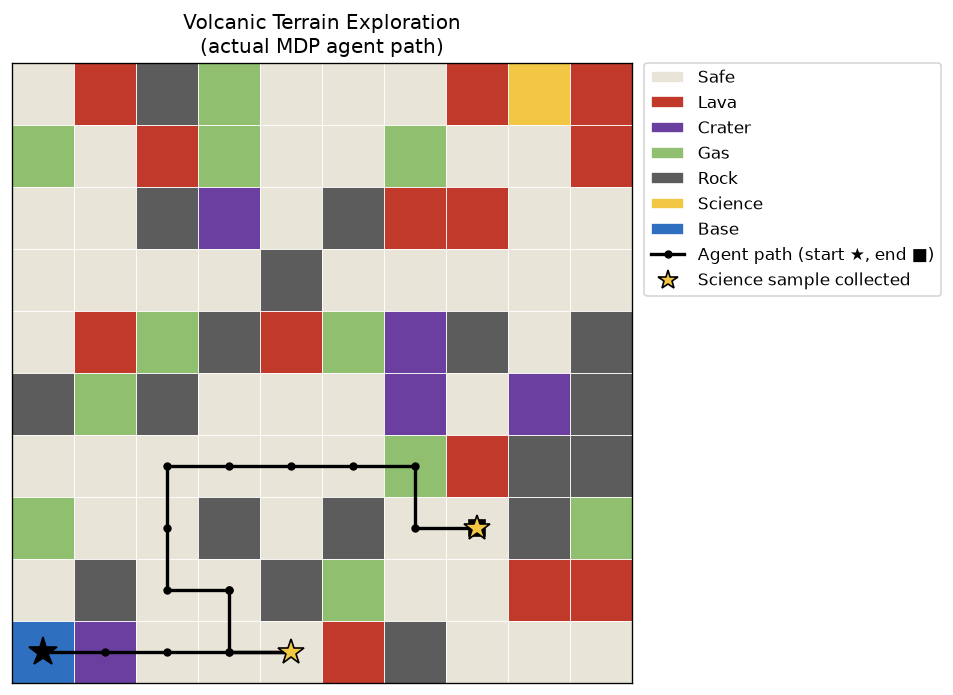
\includegraphics[width=0.72\textwidth]{final_map.png}
  \caption{Mission map for seed 42 with dynamic hazards on: the solid route is the real path taken by the MDP explorer agent (start $\star$ at BASE, end $\blacksquare$), and gold stars mark the cells where science samples were collected.}
\end{figure}

\section{Experimental Evaluation}

\subsection{Setup}

Three agents were compared (\texttt{experiments.py}), all sharing the same environment, movement uncertainty, reward accounting, collect-once rule, and termination conditions --- the baselines only override action selection:

\begin{itemize}
  \item \textbf{MDP agent} --- follows the value-iteration policy with re-planning.
  \item \textbf{Greedy agent} --- breadth-first search toward the nearest unvisited cell, treating only rock and lava as impassable (ignores soft hazard costs).
  \item \textbf{Random agent} --- uniformly random movement direction.
\end{itemize}

Each agent ran on 20 independently generated terrains (seeds 0--19), 100 steps maximum per episode.

\subsection{Results}

\begin{table}[H]
  \centering
  \begin{tabular}{lrrrrrr}
    \toprule
    Agent & Avg.\ reward & Coverage \% & Hazards & Science & Survival \% & Steps \\
    \midrule
    MDP    & $\mathbf{42.0}$ & $13.9$          & $\mathbf{1.9}$ & $\mathbf{3.5}$ & $\mathbf{60.0}$ & $21.1$ \\
    Greedy & $-124.5$        & $\mathbf{29.3}$ & $9.0$          & $2.9$          & $30.0$          & $38.2$ \\
    Random & $-179.5$        & $7.6$           & $3.8$          & $0.7$          & $15.0$          & $21.9$ \\
    \bottomrule
  \end{tabular}
  \caption{Average performance over 20 random terrains (generated by \texttt{python support/experiments.py}).}
\end{table}

\begin{figure}[H]
  \centering
  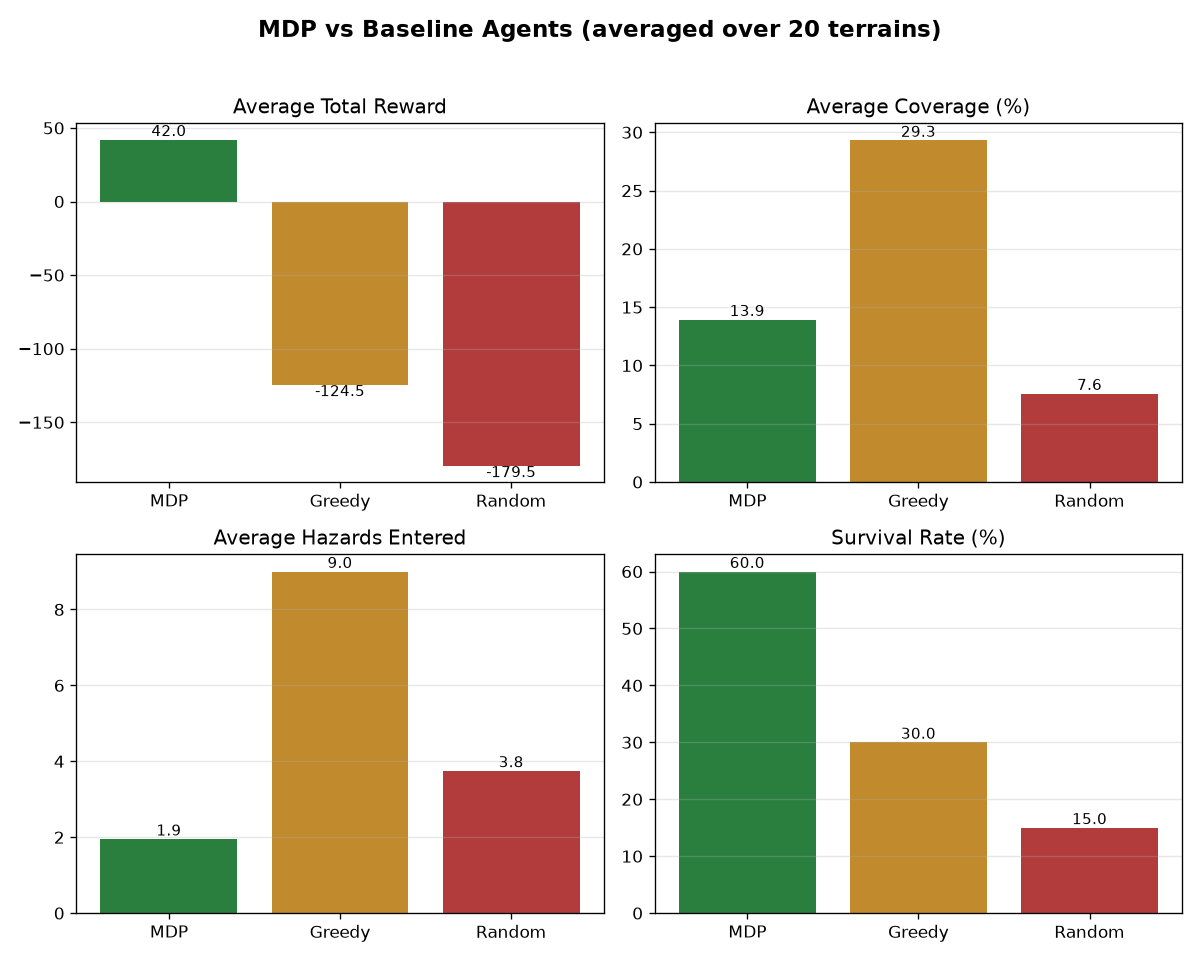
\includegraphics[width=0.85\textwidth]{performance_plot.png}
  \caption{MDP vs.\ Greedy vs.\ Random averaged over 20 terrains.}
\end{figure}

\subsection{Discussion}

\begin{itemize}
  \item The MDP agent is the only one with \textbf{positive average reward}, and it doubles the greedy baseline's survival rate while entering roughly one-fifth as many hazards.
  \item The greedy baseline achieves the highest raw coverage, but it pays for it: it marches through gas and craters and dies in 70\% of missions. Coverage without survival is not useful exploration.
  \item The MDP agent is deliberately conservative: it collects the samples whose expected value justifies the risk, then parks. This is the correct behavior under the stated reward model rather than a shortcoming of the solver.
  \item Under dynamic hazards the agent re-plans whenever the world changes; in the seed-42 demo mission it still collects its samples and survives while 71 terrain-change events occur around it.
\end{itemize}

\section{Limitations and Future Work}

\begin{itemize}
  \item Movement noise and hazard dynamics use fixed hand-chosen probabilities; learning them from data (or exposing them in the config) would make the model richer.
  \item The state is position-only. Adding remaining-science or energy to the state would let the planner reason about them exactly instead of via re-planning.
  \item The agent is risk-neutral; a risk-sensitive objective (e.g., penalizing variance or using a survival constraint) could raise the survival rate further.
  \item Partial observability (fog of war with \textsc{scan} revealing cells) would turn the problem into a POMDP --- a natural next step for the \textsc{scan} action, which is currently priced but rarely useful.
\end{itemize}

\section{Conclusion}

The project delivers a complete MDP-based exploration stack: seeded volcanic terrain generation, an exact value-iteration planner, a stochastic explorer agent with collect-once re-planning, dynamic hazards that force on-line adaptation, and a reproducible experimental comparison. The MDP agent decisively outperforms random and greedy baselines on reward, safety, and survival, demonstrating that sequential decision-theoretic planning is the right tool for hazardous exploration.

\appendix

\section{Reproducing Every Result}

\begin{verbatim}
pip install -r requirements.txt
python main.py                       # full pipeline, dynamic hazards ON
python main.py --static --seed 7     # static terrain, different map
python support/experiments.py        # baseline comparison (CSV + plot)
python support/demo_video.py         # animated demo video
\end{verbatim}

\end{document}
